\section{Elektrochemie}

\subsection{Galvanische Zellen}

\subsubsection{Grundprinzip}
Oxidation und Reduktion sind räumlich getrennt, dh. die übertragenen Elektronen können genutzt werden, um Arbeit zu leisten (elektrochemische Stromerzeugung).\\
\textbf{Elektrode:} Elektronenleiter, der Teil einer galv. Zelle ist. Meist handelt es sich dabei um ein Metall oder um Graphit.\\
\textbf{Anode:} Ort der Oxidation \\
\textbf{Kathode:} Ort der Reduktion \\
\textbf{Elektrolyt(lösung):} Stoff, der bewegliche Ionen enthält.\\
\textbf{Salzbrücke:} Sie ermöglicht den freien Fluss von Ionen zwischen den Elektrolyt-Lösungen. Im Falle eines aus zwei Halbzellen bestehenden galvanisches Elementes verhindert die Salzbrücke den Aufbau von Ladung in den Halbzellen, welche den Stromfluss ansonsten frühzeitig zum Erliegen bringen würde.\\
\textbf{Diaphragma:} Manchmal wird anstelle einer Salzbrücke ein Diaphragma verwendet. Dabei handelt es sich um eine dünne, halbdurchlässige Membran oder im einfacheren Fall um eine poröse, filterähnliche Trennwand. Verhindert die Vermischung der beiden Lösungen, garantiert aber die Ionenwanderung zwischen den Halbzellen.

\subsubsection{Das Daniell-Element}
Das Daniell-Element besteht aus einer Zink- (Zinkblech in Zinksalz-Lösung) und einer Kupfer-Halbzelle (Kupferblech in Kupfersalz-Lösung). An der Kupferelektrode (+0.34V) herrscht ein geringerer Elektronendruck als an der Zinkelektrode (-0.76V). Verbindet man die beiden Bleche, so werden Elektronen vom Ort mit dem höheren Elektronendruck (Zink) zum Ort mit dem niedrigen Elektronendruck (Kupfer) verschoben.\\
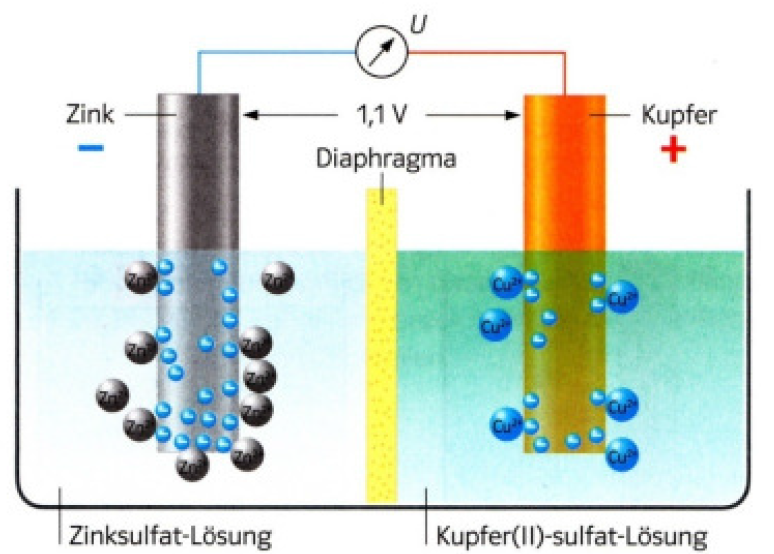
\includegraphics[width=0.7\linewidth]{images/10_Daniell_Element.png}

Spannung $\Delta E = E_\text{Kathode}-E_\text{Anode}$ \\

\textbf{Reaktionen:}\\
Zink-Halbzelle (Anode): $Zn \rightarrow Zn^{2+} + 2 e^-$ \\
Kupfer-Halbzelle (Kathode): $Cu^{2+} + 2 e^- \rightarrow Cu$ \\
Gesamtreaktion: $Zn + Cu^{2+} \rightarrow Zn^{2+} + Cu$\\

\textbf{Verkürzte Schreibweise einer Galvanischen Zelle:}\\
$Zn/Zn^{2+} // Cu^{2+}/Cu$\\
Der einfache Schrägstrich bedeutet Phasengrenze. Der doppelte kennzeichnet die Salzbrücke bzw. das Diaphragma.

\subsubsection{Standard-Wasserstoffelektrode}
Referenzmessung des Redoxpotentials

\begin{figure}[htbp!]
	\centering
	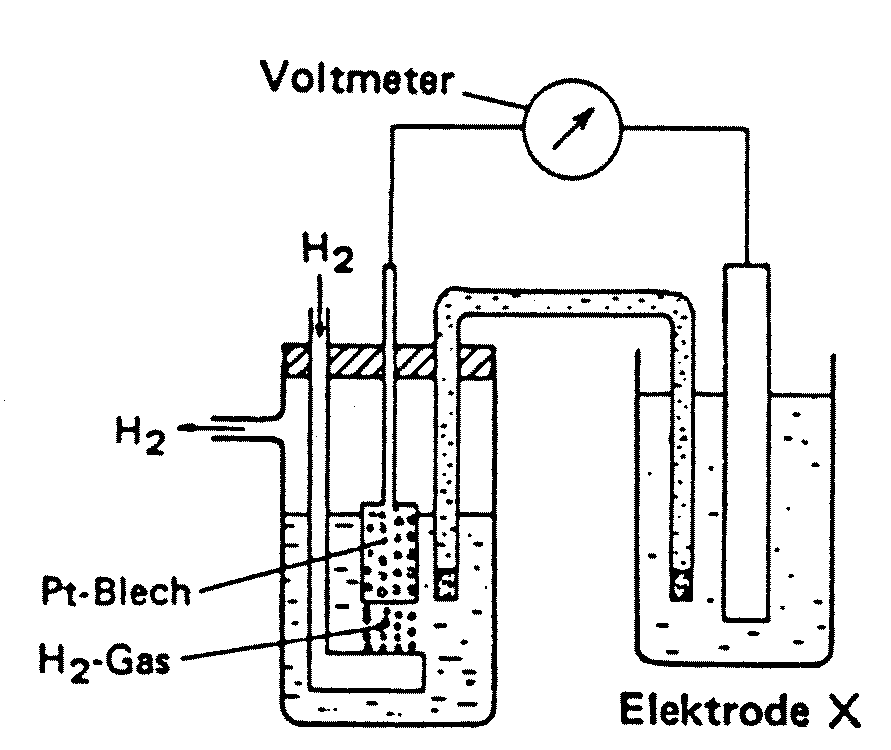
\includegraphics[width=0.6\linewidth]{images/10_Wasserstoffelektrode.png}
\end{figure}

Standardbedingungen:\\
p($H_2$) = 1013mbar, T=25$^\circ C$, Konzentration $[H_3O^+]$ = 1mol/l, $E^0(H_2/H_3O^+) = 0.0V$

Reaktionen: \\
Wasserstoff-Halbzelle: $H_2 + 2H_2O \leftrightarrow 2 H_3O^+ + 2 e^-$ \\
Halbzelle: $Me^{z+} + z e^- \leftrightarrow Me_{(s)}$

\subsection{Batterien}
Batterien sind galvanische Zellen, welche nach der Entladung nicht erneut aufgeladen werden können.

\subsubsection{Zink-Braunstein-Zelle}
\textbf{Anode:} Zinkbecher\\
\textbf{Kathode:} Braunstein($MnO_2$)/Graphit-Mischung und ein Kohlestab (nimmt nicht an der Reaktion teil). Graphit wird hinzugefügt, damit Mischung leitend wird.\\ 
\textbf{Elektrolyt:} Pappe, welche in einer $NH_4Cl$-Lösung (sauer) getränkt ist. Diese wirkt gleichzeitig als Diaphragma.\\\\

Reaktionen: \\
Anode (Ox): $Zn \rightarrow Zn^{2+}+2e^-$\\
Kathode (Red): $2MnO_2+2H_3O^++2e^- \rightarrow 2MnO(OH)+2H_2O$\\
Gesamtreaktion: $Zn+2MnO_2+2H_3O^+ \rightarrow 2MnO(OH)+Zn^{2+}+2H_2O$\\\\
Eine Zink-Braunstein-Zelle weist eine Spannung von ca. 1.5V auf.\\

Nachteile: nicht auslaufsicher, nicht hochstrombelastbar, hohe Selbstentladung

\subsubsection{Alkali-Mangan-Batterie}
Gleiche Reaktion wie bei Zink-Braunstein-Zelle. Elektrolyt: Kalilauge ($KOH
$, alkalisch). Vorteile: auslaufsicherer, günstigeres Entladeverhalten, pro $Ah$ ca. halb so teuer.

